\section{Comparaison de combustibles}\label{ex:comparaison}

\begin{center}
	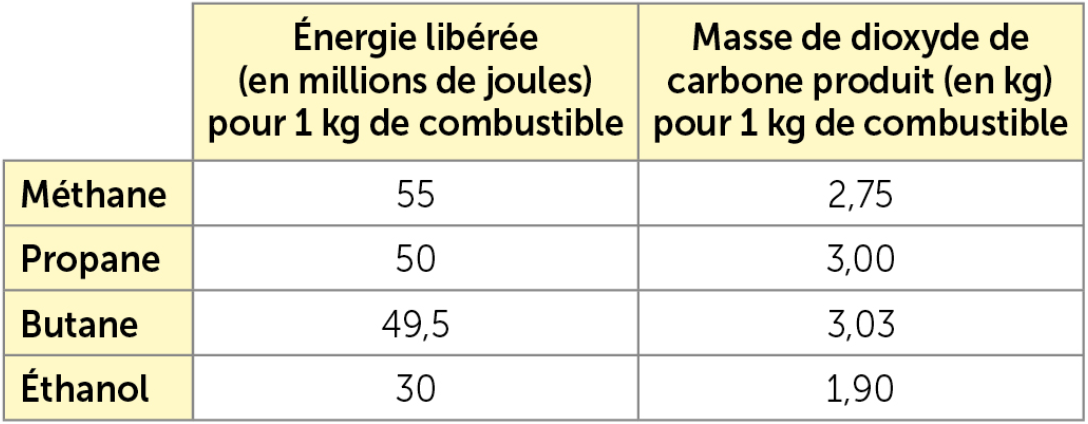
\includegraphics[scale=0.5]{img/tab_combustibles}
\end{center}

\begin{questions}
	\question Quel est le combustible le plus rentable énergiquement ?
		\begin{solution}
			Le méthane est le combustible le plus rentable énergiquement, c'est celui qui libère le plus d'énergie pour 1 kg consommé.
		\end{solution}
	
	\question Sachant que le dioxyde de carbone est un gaz à effet de serre qui contribue au réchauffement climatique, quel combustible est le plus écologique ?
		\begin{solution}
			L'éthanol est le combustible le plus écologique, c'est celui qui produit le moins de dioxyde de carbone pour 1 kg consommé.
		\end{solution}
	
	\question Calculer la quantité d'énergie libérée par la combustion de 60 kg de propane et la masse de dioxyde de carbone produit.
		\begin{solution}
			La combustion de 60 kg de propane libère \num{3000} millions de joules ($50 \times 60$) et produit \num{180} kg de dioxyde de carbone ($60 \times 3$).
		\end{solution}
\end{questions}